\documentclass[specification,annotation,times]{itmo-student-thesis}

%% Опции пакета:
%% - specification - если есть, генерируется задание, иначе не генерируется
%% - annotation - если есть, генерируется аннотация, иначе не генерируется
%% - times - делает все шрифтом Times New Roman, собирается с помощью xelatex
%% - pscyr - делает все шрифтом Times New Roman, требует пакета pscyr.

%% Делает запятую в формулах более интеллектуальной, например:
%% $1,5x$ будет читаться как полтора икса, а не один запятая пять иксов.
%% Однако если написать $1, 5x$, то все будет как прежде.
\usepackage{icomma}

%% Один из пакетов, позволяющий делать таблицы на всю ширину текста.
\usepackage{tabularx}

%% Данные пакеты необязательны к использованию в бакалаврских/магистерских
%% Они нужны для иллюстративных целей
%% Начало
\usepackage{tikz}
\usetikzlibrary{arrows}
%% Конец

%% Указываем файл с библиографией.
\addbibresource{master-thesis.bib}

\begin{document}

\studygroup{M4239}
\title{Децентрализованный алгоритм управления конвейерной системой с использованием методов мультиагентного обучения с подкреплением}
\author{Мухутдинов Дмитрий Вадимович}{Мухутдинов Д.В.}
\supervisor{Фильченков Андрей Александрович}{Фильченков А.А.}{к.ф-м.н.}{кафедра КТ}
\publishyear{2019}
%% Дата выдачи задания. Можно не указывать, тогда надо будет заполнить от руки.
\startdate{01}{сентября}{2017}
%% Срок сдачи студентом работы. Можно не указывать, тогда надо будет заполнить от руки.
\finishdate{31}{мая}{2019}
%% Дата защиты. Можно не указывать, тогда надо будет заполнить от руки.
\defencedate{07}{июня}{2019}

\addconsultant{Вяткин В.В.}{проф., д.т.н.}

\secretary{Павлова О.Н.}

%% Задание
%%% Техническое задание и исходные данные к работе
\technicalspec{Требуется разработать децентрализованный алгоритм управления
  конвейерной системы для транспортировки багажа. Алгоритм должен позволять
  контроллерам конвейерной сети динамически изменять свое поведение в целях
  адаптации под изменившиеся условия работы, такие как поломка одного из
  конвейеров или изменение интенсивности потока багажа. Алгоритм должен
  обеспечивать своевременную доставку багажных единиц до пунктов назначения, в
  то же время минимизируя энергопотребление всей системы в целом.
}

%%% Содержание выпускной квалификационной работы (перечень подлежащих разработке вопросов)
\plannedcontents{Пояснительная записка должна содержать обзор существующих
  результатов в сфере управления конвейерными системами, а также в сферах,
  имеющих непосредственное отношение к предложенному алгоритму (таких как
  сетевая маршрутизация и обучение с подкреплением). Также записка должна
  содержать подробное изложение предложенного алгоритма и данные
  экспериментального сравнения его производительности с производительностью
  существующих методов управления конвейерной системой, проведенного с помощью
  виртуальной имитационной модели конвейерной сети.
}

%%% Исходные материалы и пособия 
\plannedsources{\begin{enumerate}
  \item Richard S. Sutton and Andrew G. Barto. Reinforcement Learning: An Introduction. The MIT Press, 2012
  \item Mnih et al. Human-level control through deep reinforcement learning. Nature, 518(7540):529–533, 2015.
\end{enumerate}}

%%% Календарный план
%% \addstage{Ознакомление с предметной областью}{11.2017}
%% \addstage{Чтение статей, посвященных алгоритмам маршрутизации}{01.2018}
%% \addstage{Чтение статей, посвященных задаче обучения с подкреплением}{02.2018}
%% \addstage{Чтение статей, посвященных задаче обучения с подкреплением}{03.2018}
%% \addstage{Чтение статей, посвященных задаче управления конвейерными системами}{05.2018}
%% \addstage{Разработка имитационной модели конвейерной сети}{09.2018}
%% \addstage{Реализация существующих алгоритмов управления}{11.2018}
%% \addstage{Разработка алгоритма маршрутизации, проведение экспериментов}{03.2019}
%% \addstage{Написание пояснительной записки}{05.2019}

%%% Цель исследования
\researchaim{
  Разработка децентрализованного алгоритма управления конвейерной системой,
  способного адаптироваться к гетерогенным изменениям в условиях работы.
}

%%% Задачи, решаемые в ВКР
\researchtargets{\begin{enumerate}
    \item разработка виртуальной имитационной модели конвейерной сети,
      позволяющей проводить сравнительный анализ алгоритмов управления;
    \item реализация ряда известных алгоритмов управления конвейерной сетью (а
      также маршрутизации) в рамках разработанной имитационной модели;
    \item разработка алгоритма, соответствующего поставленным требованиям;
    \item экспериментальное сравнение разработанного алгоритма с существующими
      по качеству работы.
\end{enumerate}}

%%% Использование современных пакетов компьютерных программ и технологий
\addadvancedsoftware{Язык программирования Python 3.6}{}
\addadvancedsoftware{Библиотека для дискретно-событийного моделирования SimPy}{}
\addadvancedsoftware{Библиотека для операций с графами NetworkX}{}
\addadvancedsoftware{Математические пакеты NumPy и SciPy}{}
\addadvancedsoftware{Библиотеки для машинного обучения scikit-learn и PyTorch}{}
\addadvancedsoftware{Среда интерактивной разработки Jupyter Lab}{}
\addadvancedsoftware{Библиотеки Matplotlib, Seaborn и Pandas для обработки и визуализации данных}{}

%%% Краткая характеристика полученных результатов 
\researchsummary{
  Разработан алгоритм управления конвейерной системой на основе глубокого
  мультиагентного обучения с подкреплением. В ходе экспериментального
  исследования было установлено, что разработанный алгоритм превосходит
  существующие по качеству работы и способен адаптироваться к изменениям во
  внешней среде.
}

%%% Гранты, полученные при выполнении работы 
\researchfunding{
  Государственное задание № 2.8866.2017/БЧ <<Технология разработки программного
  обеспечения систем управления ответственными объектами на основе глубокого
  обучения и конечных автоматов>>
}

%%% Наличие публикаций и выступлений на конференциях по теме выпускной работы
\researchpublications{
\begin{refsection}
\nocite{mukhutdinov2019multi}
\printannobibliography
\end{refsection}
}

%% Эта команда генерирует титульный лист и аннотацию.
\maketitle{Магистр}

%% Оглавление
\tableofcontents

%% Макрос для введения. Совместим со старым стилевиком.
\startprefacepage

Конвейерные системы широко применяются для автоматизированной транспортировки
объектов и материалов. Они являются неотъемлемой частью комплексов промышленного
оборудования, пунктов сортировки грузов, багажных систем в аэропортах и т. д..
Оптимизация работы таких системы имеет высокую практическую и экономическую
значимость, что мотивирует поиск эффективных методов управления конвейерными
системами.

Для управления большинством современных конвейерных систем применяются
централизованные статические стратегии управления, специально разрабатываемые
под конкретную систему одновременно с проектированием ее физической топологии в
целях решения задач конкретного предприятия \cite{de1994baggage}. Преимуществами
такого подхода являются высокая производительность работы и предсказуемость
поведения системы. Недостатками такого подхода являются высокая стоимость и
долгие сроки разработки кастомизированной стратегии управления, неспособность
системы адаптироваться к изменениям во внешний условиях, не учтенных во время
проектирования (таким как неожиданный отказ отдельных элементов системы), а
также наличие централизованного контроллера как критической точки отказа.

В связи с обозначенными недостатками использования кастомизированных стратегий
управления существует интерес к разработке обобщенных систематических подходов к
управлению конвейерными системами. Наиболее популярным подходом из используемых
является управление с прогнозируемыми моделями (\textit{англ.} model predictive
control, MPC) \cite{qin2003survey}. Управление с прогнозируемыми моделями
изначально разрабатывалось для задач химической промышленности и
нефтепереработки \cite{eaton1992model}, и на данный момент широко используется в
этих сферах. В последние несколько лет повысился интерес к применению данного
подхода к управлению другими типами киберфизических систем, в том числе
промышленными конвейерными линиями \cite{cataldo2016dynamic, luo2015energy} и
системами распределения багажа на основе рельсовых тележек (\textit{англ.}
destination coded vehicles, DCVs) \cite{tarau2010model, zeinaly2015integrated}.
Существующие алгоритмы на основе управления с прогнозируемыми моделями
обобщаются на различные конкретные конфигурации физических систем, но все еще
предусматривают наличие централизованного контроллера. Кроме того, модификация
существующего алгоритма управления (например, добавления учета энергопотребления
системы) во многих случаях является нетривиальной задачей, так как
оптимизируемая функция во фреймворке MPC должна выражаться как задача линейного
(\textit{англ.} linear programming, LP) или квадратичного программирования
(\textit{англ.} quadratic programming, QP). В связи с этим существует интерес к
разработке иных, децентрализованных подходов к управлению конвейерными сетями,
требующих менее строгих ограничений к характеру решаемой задачи.

При рассмотрении штучных конвейеров, перемещающих отдельные объекты, как в
случае систем для перемещения багажа в аэропортах, задача управления конвейерной
системой по большей части сводится к задаче пакетной маршрутизации
(\textit{англ.} packet routing). Задача пакетной маршрутизации --- это задача
поиска пути наименьшей стоимости в графе из текущей вершины $n$ в вершину
назначения $d$. В контексте конвейерных систем топология конвейерной сети может
быть представлена в виде ориентированного графа, а перемещаемые по конвейерам
объекты могут быть абстрагированы как <<пакеты>>. 

Задача пакетной маршрутизации впервые обрела актуальность с появлением
компьютерных сетей. Первые алгоритмы сетевой маршрутизации появились в процессе
разработки сети ARPANet. Именно тогда были изобретены такие подходы к пакетной
маршрутизации, как дистанционно-векторный (\textit{англ.} distance-vector)
\cite{arpanet-orig} и состояния каналов связи (\textit{англ.} link-state)
\cite{link-state-arpanet}, которые и по сей день лежат в основе
таких стандартных и широко применяемых алгоритмов сетевой маршрутизации, как
Routing Information Protocol (RIP) \cite{rip-rfc} и Open Shortest Path First
(OSPF) \cite{ospf-rfc}. Преимуществами алгоритмов сетевой маршрутизации являются
обусловленные характером задачи децентрализованность, низкая требовательность к
вычислительным ресурсам и устойчивость к отказам маршрутизаторов и обрывам
соединений. В работе \cite{vyatkin-controllers} было продемонстрировано, что
простой дистанционно-векторный алгоритм маршрутизации может быть напрямую
применен к задаче управления конвейерной системой для транспортировки багажа,
что позволяет достигнуть устойчивости системы к отказам отдельных конвейеров.
Однако, в силу своей простоты, дистанционно-векторный алгоритм решает
исключительно задачу направления перемещаемых объектов вдоль кратчайших путей в
конвейерной сети, что ограничивает его применимость в тех случаях, когда
необходимо учитывать дополнительные критерии оптимизации (такие как
энергопотребление системы).

Cуществуют и другие подходы к решению задачи пакетной маршрутизации. Одним из
таких подходов является подход на основе идеи обучения с подкреплением
(\textit{англ.} reinforcement learing, RL). Первым таким алгоритмом стал алгоритм
Q-routing \cite{q-routing-orig}, основанный на методе Q-learning
\cite{q-learning-orig}. Этот алгоритм, как и его модификации
\cite{predictive-q-routing, dual-q-routing}, благодаря обучению с подкреплением
оказался способен лучше адаптироваться к изменениям в интенсивности сетевого
трафика, чем алгоритмы, основанные на вычислении кратчайшего пути. Но из-за
использования большого количества служебных сообщений, использующих те же каналы
передачи данных, что и целевые пакеты, применение таких алгоритмов в реальных
компьютерных сетях ограничено.

В контексте конвейерных сетей, однако, целевые <<пакеты>> являются физическими
объектами (например, чемоданами), перемещаемыми по конвейерной ленте, в то время
как служебные сообщения передаются по проводным соединениям между контроллерами.
Таким образом, время распространения служебных сообщений по системе пренебрежимо
мало по сравнению с временем перемещения целевых объектов, что нивелирует
озвученный недостаток алгоритмов маршрутизации, основанных на обучении с
подкреплением.

В данной работе будет предложено несколько модификаций децентрализованного
алгоритма управления конвейерной системой, основанного на методе Q-routing, но
использующего нейронную сеть в качестве обучающегося агента. Для демонстрации
способности работы алгоритма в различных постановках задачи маршрутизации он
будет исследован как в имитационной модели конвейерной системы, так и в
имитационной модели абстрактной компьютерной сети.

В главе 1 будет сформулирована обобщенная постановка задачи маршрутизации в
терминах мультиагентного обучения с подкреплением, к которой будет сведена
задача управления конвейерной системой. Будут рассмотрены существующие
алгоритмы маршрутизации, их сильные и слабые стороны. Также будут рассмотрены
существующие методы обучения нейронных сетей с подкреплением, в том числе в
мультиагентном случае.

В главе 2 будет рассмотрен предложенный алгоритм и его модификации и обоснованы
решения, принятые в ходе его разработки.

В главе 3 будут приведены экспериментальные результаты работы алгоритма для
задач пакетной маршрутизации в моделях компьютерной сети и управления системой багажных
конвейеров. Также будет проведено экспериментальное сравнение алгоритма с
существующими алгоритмами маршрутизации и управления конвейерной системой.

%% Начало содержательной части.
\chapter{Первая глава}

%% Так помечается начало обзора.
\startrelatedwork
Пример ссылок в рамках обзора: \cite{vyatkin-controllers, q-routing-orig, tan1993multi}.
%% Так помечается конец обзора.
\finishrelatedwork
Вне обзора:~\cite{bellman-ford}.

\section{Таблицы}

В качестве примера таблицы приведена таблица~\ref{tab1}.

\begin{table}[!h]
\caption{Таблица умножения (фрагмент)}\label{tab1}
\centering
\begin{tabular}{|*{18}{c|}}\hline
-- & 1 & 2 & 3 & 4 & 5 & 6 & 7 & 8 & 9 & 10 & 11 & 12 & 13 & 14 & 15 & 16 & 17 \\\hline
1  & 1 & 2 & 3 & 4 & 5 & 6 & 7 & 8 & 9 & 10 & 11 & 12 & 13 & 14 & 15 & 16 & 17 \\\hline
2  & 2 & 4 & 6 & 8 & 10 & 12 & 14 & 16 & 18 & 20 & 22 & 24 & 26 & 28 & 30 & 32 & 34 \\\hline
3  & 3 & 6 & 9 & 12 & 15 & 18 & 21 & 24 & 27 & 30 & 33 & 36 & 39 & 42 & 45 & 48 & 51 \\\hline
4  & 4 & 8 & 12 & 16 & 20 & 24 & 28 & 32 & 36 & 40 & 44 & 48 & 52 & 56 & 60 & 64 & 68 \\\hline
\end{tabular}
\end{table}

Есть еще такое окружение \texttt{tabularx}, его можно аккуратно растянуть на всю страницу.
Приведем пример (таблица~\ref{tab2}).

\begin{table}[!h]
\caption{Таблица умножения с помощью \texttt{tabularx} (фрагмент)}\label{tab2}
\centering
\begin{tabularx}{\textwidth}{|*{18}{>{\centering\arraybackslash}X|}}\hline
-- & 1 & 2 & 3 & 4 & 5 & 6 & 7 & 8 & 9 & 10 & 11 & 12 & 13 & 14 & 15 & 16 & 17 \\\hline
1  & 1 & 2 & 3 & 4 & 5 & 6 & 7 & 8 & 9 & 10 & 11 & 12 & 13 & 14 & 15 & 16 & 17 \\\hline
2  & 2 & 4 & 6 & 8 & 10 & 12 & 14 & 16 & 18 & 20 & 22 & 24 & 26 & 28 & 30 & 32 & 34 \\\hline
3  & 3 & 6 & 9 & 12 & 15 & 18 & 21 & 24 & 27 & 30 & 33 & 36 & 39 & 42 & 45 & 48 & 51 \\\hline
4  & 4 & 8 & 12 & 16 & 20 & 24 & 28 & 32 & 36 & 40 & 44 & 48 & 52 & 56 & 60 & 64 & 68 \\\hline
\end{tabularx}
\end{table}

\section{Рисунки}

Пример рисунка (c помощью \texttt{TikZ}) приведен на рисунке~\ref{fig1}. Под \texttt{pdflatex} можно также
использовать \texttt{*.jpg}, \texttt{*.png} и даже \texttt{*.pdf}, под \texttt{latex} можно использовать
Metapost. Последний можно использовать и под \texttt{pdflatex}, для чего в стилевике продекларированы
номера картинок от~1 до~20.

\begin{figure}[!h]
\caption{Пример рисунка}\label{fig1}
\centering
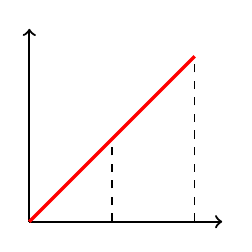
\begin{tikzpicture}[scale=0.7]
\draw[thick,->] (0,0)--(3.5,0);
\draw[thick,->] (0,0)--(0,3.5);
\draw[very thick, red] (0,0)--(3,3);
\draw[dashed] (3,0)--(3,3);
\draw[dashed] (1.5,0)--(1.5,1.5);
\end{tikzpicture}
\end{figure}

\section{Листинги}

В работах студентов кафедры <<Компьютерные технологии>> часто встречаются листинги. Листинги бывают
двух основных видов~--- исходный код и псевдокод. Первый оформляется с помощью окружения \texttt{lstlisting}
из пакета \texttt{listings}, который уже включается в стилевике и немного настроен. Пример Hello World на Java
приведен на листинге~\ref{lst1}. Пример большого листинга~--- в приложении (листинг~\ref{lstX}).

\begin{lstlisting}[float=!h,caption={Пример исходного кода на Java},label={lst1}]
public class HelloWorld {
	public static void main(String[] args) {
		System.out.println("Hello, world!");
	}
}
\end{lstlisting}

Псевдокод можно оформлять с помощью разных пакетов. В данном стилевике включается пакет \texttt{algorithmicx}.
Сам по себе он не генерирует флоатов, поэтому для них используется пакет \texttt{algorithm}.
Пример их совместного использования приведен на листинге~\ref{lst2}.

\begin{algorithm}[!h]
\caption{Пример псевдокода}\label{lst2}
\begin{algorithmic}
	\Function{IsPrime}{$N$}
		\For{$t \gets [2; \lfloor\sqrt{N}\rfloor]$}
			\If{$N \bmod t = 0$}
				\State\Return \textsc{false}
			\EndIf
		\EndFor
		\State\Return \textsc{true}
	\EndFunction
\end{algorithmic}
\end{algorithm}

Наконец, листинги из \texttt{listings} тоже можно подвешивать с помощью \texttt{algorithm},
пример на листинге~\ref{lst3}.

\begin{algorithm}[!h]
\caption{Исходный код и флоат \texttt{algorithm}}\label{lst3}
\begin{lstlisting}
public class HelloWorld {
	public static void main(String[] args) {
		System.out.println("Hello, world!");
	}
}
\end{lstlisting}
\end{algorithm}

\chapter{Проверка сквозной нумерации}

Листинг~\ref{lst4} должен иметь номер 4.

\begin{algorithm}[!h]
\caption{Исходный код и флоат \texttt{algorithm}}\label{lst4}
\begin{lstlisting}
public class HelloWorld {
	public static void main(String[] args) {
		System.out.println("Hello, world!");
	}
}
\end{lstlisting}
\end{algorithm}

Рисунок~\ref{fig2} должен иметь номер 2.

\begin{figure}[!h]
\caption{Пример рисунка}\label{fig2}
\centering
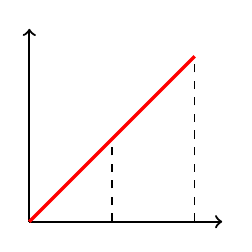
\begin{tikzpicture}[scale=0.7]
\draw[thick,->] (0,0)--(3.5,0);
\draw[thick,->] (0,0)--(0,3.5);
\draw[very thick, red] (0,0)--(3,3);
\draw[dashed] (3,0)--(3,3);
\draw[dashed] (1.5,0)--(1.5,1.5);
\end{tikzpicture}
\end{figure}

Таблица~\ref{tab3} должна иметь номер 3.

\begin{table}[!h]
\caption{Таблица умножения с помощью \texttt{tabularx} (фрагмент)}\label{tab3}
\centering
\begin{tabularx}{\textwidth}{|*{18}{>{\centering\arraybackslash}X|}}\hline
-- & 1 & 2 & 3 & 4 & 5 & 6 & 7 & 8 & 9 & 10 & 11 & 12 & 13 & 14 & 15 & 16 & 17 \\\hline
1  & 1 & 2 & 3 & 4 & 5 & 6 & 7 & 8 & 9 & 10 & 11 & 12 & 13 & 14 & 15 & 16 & 17 \\\hline
2  & 2 & 4 & 6 & 8 & 10 & 12 & 14 & 16 & 18 & 20 & 22 & 24 & 26 & 28 & 30 & 32 & 34 \\\hline
3  & 3 & 6 & 9 & 12 & 15 & 18 & 21 & 24 & 27 & 30 & 33 & 36 & 39 & 42 & 45 & 48 & 51 \\\hline
4  & 4 & 8 & 12 & 16 & 20 & 24 & 28 & 32 & 36 & 40 & 44 & 48 & 52 & 56 & 60 & 64 & 68 \\\hline
\end{tabularx}
\end{table}

\chapterconclusion

В конце каждой главы желательно делать выводы. Вывод по данной главе~--- нумерация работает корректно, ура!

%% Макрос для заключения. Совместим со старым стилевиком.
\startconclusionpage

В данном разделе размещается заключение.

%% Обратите внимание на heading. Без него тоже работает, но название будет другим.
\printmainbibliography

%% После этой команды chapter будет генерировать приложения, нумерованные русскими буквами.
%% \startappendices из старого стилевика будет делать то же самое
\appendix

\chapter{Пример приложения}

В приложениях рисунки, таблицы и другие подобные элементы нумеруются по приложениям с соответствующим префиксом. Проверим это.

Листинг~\ref{lst4:apx} должен иметь номер А.1.

\begin{algorithm}[!h]
\caption{Исходный код и флоат \texttt{algorithm}}\label{lst4:apx}
\begin{lstlisting}
public class HelloWorld {
    public static void main(String[] args) {
        System.out.println("Hello, world!");
    }
}
\end{lstlisting}
\end{algorithm}

Рисунок~\ref{fig2:apx} должен иметь номер A.1.

\begin{figure}[!h]
\caption{Пример рисунка}\label{fig2:apx}
\centering
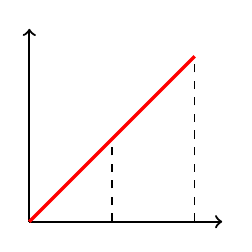
\begin{tikzpicture}[scale=0.7]
\draw[thick,->] (0,0)--(3.5,0);
\draw[thick,->] (0,0)--(0,3.5);
\draw[very thick, red] (0,0)--(3,3);
\draw[dashed] (3,0)--(3,3);
\draw[dashed] (1.5,0)--(1.5,1.5);
\end{tikzpicture}
\end{figure}

Таблица~\ref{tab3:apx} должна иметь номер A.1.

\begin{table}[!h]
\caption{Таблица умножения с помощью \texttt{tabularx} (фрагмент)}\label{tab3:apx}
\centering
\begin{tabularx}{\textwidth}{|*{18}{>{\centering\arraybackslash}X|}}\hline
-- & 1 & 2 & 3 & 4 & 5 & 6 & 7 & 8 & 9 & 10 & 11 & 12 & 13 & 14 & 15 & 16 & 17 \\\hline
1  & 1 & 2 & 3 & 4 & 5 & 6 & 7 & 8 & 9 & 10 & 11 & 12 & 13 & 14 & 15 & 16 & 17 \\\hline
2  & 2 & 4 & 6 & 8 & 10 & 12 & 14 & 16 & 18 & 20 & 22 & 24 & 26 & 28 & 30 & 32 & 34 \\\hline
3  & 3 & 6 & 9 & 12 & 15 & 18 & 21 & 24 & 27 & 30 & 33 & 36 & 39 & 42 & 45 & 48 & 51 \\\hline
4  & 4 & 8 & 12 & 16 & 20 & 24 & 28 & 32 & 36 & 40 & 44 & 48 & 52 & 56 & 60 & 64 & 68 \\\hline
\end{tabularx}
\end{table}

Заодно проверим нумерованные и ненумерованные перечисления. Ненумерованные:
\begin{itemize}
    \item пункт А;
    \item пункт Б;
    \item пункт В.
\end{itemize}

Нумерованные списки нескольких уровней:
\begin{enumerate}
    \item первый элемент;
    \item второй элемент с подэлементами:
    \begin{enumerate}
        \item первый подэлемент;
        \item второй подэлемент;
        \item третий подэлемент.
    \end{enumerate}
    \item третий элемент;
    \item четвертый элемент;
    \item пятый элемент;
    \item шестой элемент;
    \item седьмой элемент;
    \item восьмой элемент;
    \item девятый элемент;
    \item десятый элемент.
\end{enumerate}

\chapter{Еще один пример приложения с неимоверно длиннющим названием для тестирования переносов}

Проверим на примере таблиц, что нумерация в приложениях~--- по приложениям.
Таблица~\ref{tab3:apx2} должна иметь номер Б.1.

\begin{table}[!h]
\caption{Таблица умножения с помощью \texttt{tabularx} (фрагмент)}\label{tab3:apx2}
\centering
\begin{tabularx}{\textwidth}{|*{18}{>{\centering\arraybackslash}X|}}\hline
-- & 1 & 2 & 3 & 4 & 5 & 6 & 7 & 8 & 9 & 10 & 11 & 12 & 13 & 14 & 15 & 16 & 17 \\\hline
1  & 1 & 2 & 3 & 4 & 5 & 6 & 7 & 8 & 9 & 10 & 11 & 12 & 13 & 14 & 15 & 16 & 17 \\\hline
2  & 2 & 4 & 6 & 8 & 10 & 12 & 14 & 16 & 18 & 20 & 22 & 24 & 26 & 28 & 30 & 32 & 34 \\\hline
3  & 3 & 6 & 9 & 12 & 15 & 18 & 21 & 24 & 27 & 30 & 33 & 36 & 39 & 42 & 45 & 48 & 51 \\\hline
4  & 4 & 8 & 12 & 16 & 20 & 24 & 28 & 32 & 36 & 40 & 44 & 48 & 52 & 56 & 60 & 64 & 68 \\\hline
\end{tabularx}
\end{table}

\chapter{Пример огромного листинга}

\begin{lstlisting}[caption={Пример большого листинга},label={lstX}]
import java.util.*;

public class Example {
    static int[] restoreOutgoing(int[] g, int[] outgoing,
                                 int vertex, int mask) {
        int[] rv = new int[1 + Integer.bitCount(mask)];
        int n = g.length;
        int current = rv.length - 1;
        while (true) {
            rv[current] = vertex;
            if (current == 0) {
                if (vertex != 0) {
                    throw new AssertionError();
                }
                return rv;
            }
            mask ^= 1 << (vertex - 1);
            int prevMask = outgoing[mask] & g[vertex];
            if (prevMask == 0) {
                throw new AssertionError();
            }
            vertex = Integer.numberOfTrailingZeros(prevMask);
            --current;
        }
    }

    static int[] restoreIncoming(int[] g, int[] incoming,
                                 int vertex, int mask) {
        int[] rv = new int[1 + Integer.bitCount(mask)];
        int n = g.length;
        int current = 0;
        while (true) {
            rv[current] = vertex;
            if (current == rv.length - 1) {
                if (vertex != 0) {
                    throw new AssertionError();
                }
                return rv;
            }
            mask ^= 1 << (vertex - 1);
            int nextMask = incoming[mask] & g[vertex];
            if (nextMask == 0) {
                throw new AssertionError();
            }
            vertex = Integer.numberOfTrailingZeros(nextMask);
            ++current;
        }
    }
}
\end{lstlisting}
                

\end{document}
